\documentclass[fleqn]{jbook}
\usepackage{physpub}

\begin{document}

\begin{question}{専攻 問題8}{}

\begin{subquestions}
\SubQuestion
  同種のアミノ酸からなるポリペプチド鎖(ホモポリペプチド鎖)のヘリックス
  −コイル転移について考えてみよう。ヘリックス−コイル転移のジッパー
  モデル(zipper model)では、鎖中に連続した一個のヘリックスセグメント
  のみが許される。つまり \mbox{…ccchhhhhccc…}や\mbox{…hhhhhcccccc…}
  のコンフォメーションは許されるが、\\\mbox{…hhhhhcccchhhh…}や
  \mbox{…ccchhhhccchhhhhcchhhcccc…}などは許されない (ここで、hとcは、
  それぞれ、ヘリックス状態とコイル状態にある残基を表す)。このとき、
  残基数$n$ からなる鎖の分配関数$Z$ はどのように表されるか。但し、
  ヘリックス−コイル転移の開始パラメータ$\sigma$、伸長パラメータ$s$ と
  おき、各残基に対して: (1)コイル状態の統計重率は1とし;(2)コイル状態
  に続くヘリックスの統計重率は$\sigma \times s$とし;(3)ヘリックス状態
  に続くヘリックスの統計重率は$s$とせよ。また、鎖の末端はコイル状態に
  つながっているのと等価と考えよ。

\SubQuestion
  分子量2万以下の単一ドメインからなる球状タンパク質のアンフォールディ
  ング転移は、多くの場合、二状態転移で表され、各タンパク質分子は転移
  領域で天然状態(N状態)とアンフォールドした状態(U状態)のいずれか二つの
  状態しか取ることができない。これは合成ポリペプチド鎖のヘリックス−
  コイル転移が、転移領域で取り得る各分子の状態を考えたときに、多状態の
  転移であることと対照的である。球状タンパク質と合成ポリペプチド鎖の
  このような違いをもたらす物理的要因は何か。「球状タンパク質の天然構造
  」と「合成ポリペプチド鎖のヘリックス構造」の特徴に着目して答えよ。

\SubQuestion
  図1は、ある球状タンパク質の熱によるアンフォールディング転移を表し、
  縦軸はU状態の割合($f$)、横軸は温度($T$)を示す。アンフォールディング
  転移が二状態転移 N$\leftrightarrow$U で表されるとすると、転移の平衡
  定数 $K$ と転移に伴う標準自由エネルギーの変化 $\IDelta G$ はどのよう   にして求められるか。

\SubQuestion
  図1に示されたタンパク質の熱によるアンフォールディング転移のエンタル
  ピーの変化 $\IDelta H$ は、圧力一定の条件下では、
  $\IDelta H =-R \Partial{\ln K}{(1/T)}$ により得られることを示せ。
  ここで、$R$ は気体定数とする。

\SubQuestion
  図2は、図1より得られた平衡定数 $K$ の対数を温度の逆数 ($1/T$)に
  対してプロットしたものであり、ファントホッフのプロットという。
  水溶液中での球状タンパク質のアンフォールディング転移のファント
  ホッフのプロットは、一般に、直線ではなく、図2のように上に凹の曲率を
  示す。この事実から、タンパク質の天然構造を安定化している相互作用に
  関しどのようなことがいえるか。タンパク質を構成するアミノ酸を非極性
  溶媒中より水中に移すときの移行(transfer)の自由エネルギーの温度依存
  との関連に触れつつ述べよ。

\end{subquestions}

\begin{center}
  \mbox{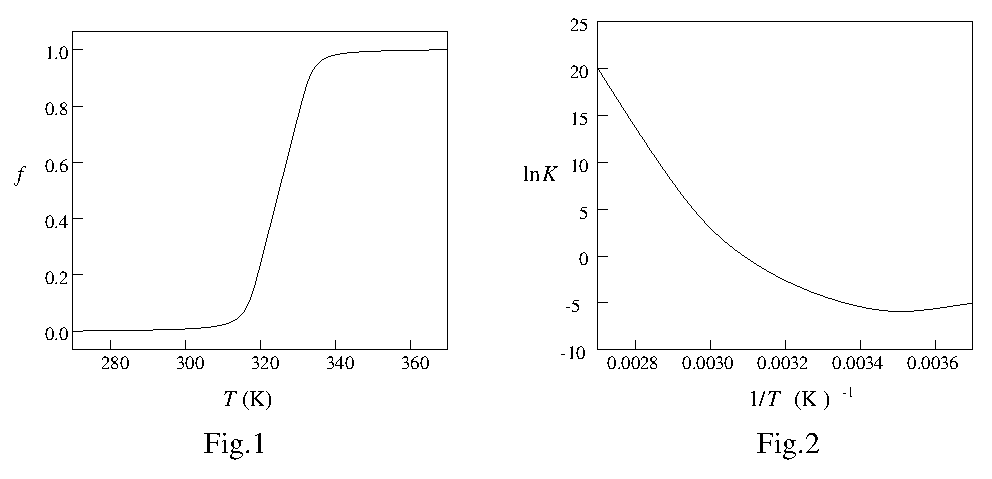
\includegraphics[clip]{1995phy8-1.eps}}
\end{center}

\end{question}
\begin{answer}{専攻 問題8}{}
\begin{subanswers}
\SubAnswer
  ジッパーモデルでは、鎖中に連続したヘリックス部分が一ヶ所のみ
  許される。すべてのコンフォーメーションを考えて、統計重率を計算する。
%
  \begin{center}
  \begin{tabular}{cccl}
  コンフォーメーション &ヘリックスの数&統計重率    &     \\
  …cccc…             &   0          &  1         &1通り\\
  …cchcc…            &   1          &$\sigma s$  &$n$通り\\
  …cchhcc…           &   2          &$\sigma s^2$&$(n-1)$通り\\
  …cch‥hcc…         &  $ k $       &$\sigma s^k$&$(n-k+1)$通り
  \end{tabular}
  \end{center}
%
  これらをすべてサムアップすると、分配関数$Z$は
%
  \begin{eqnarray*}  
    Z &=& 1 + n \sigma s + (n-1)\sigma s^2%
        + \cdots +(n-k+1)\sigma s^k + \cdots + \sigma s^n \\
      &=& 1 + \sum_{k=1}^n (n-k+1)\sigma s^k%
       =  1 + \frac{\sigma s^2 [s^n + \frac{n}{s} - (n-1)]}{(s-1)^2}
  \end{eqnarray*} 

\SubAnswer
  球状タンパク質の天然状態は、水素結合や、ジルフィス結合、疎水性相互
  作用などの様々な力による大きな安定性と大きな不安定性の微妙なバランス
  によって保たれている。そのため、ちょっとした構造の''くずれ''でも
  全体のバランスを失い、構造が急激にアンフォールディング状態へと変化
  してしまう。\\
  一方、ポリペプチド鎖のヘリックス構造は、数残基離れた、N-HとC=Oが
  水素結合をすることにより成り立っている。ランダムコイル状態の
  ポリペプチド鎖に最初のヘリックスの核ができるには、数残基が正しく
  固定される必要があるので、難しい。ところが、一度核が形成されると
  後に続くヘリックスは、一つの残基を固定するだけでヘリックス構造に
  なることができる。このようにして合成ポリペプチド鎖の
  ヘリックス−コイル転移は、多くの状態をとる。

\begin{center}
  \mbox{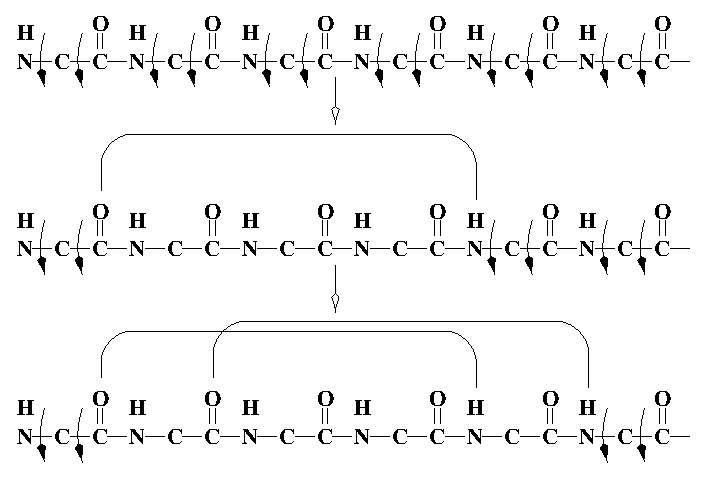
\includegraphics[clip]{1995phy8-2.eps}}
\end{center}

\newpage
\SubAnswer
  天然状態(Natural)での$1\Unit{mol}$当たりのエネルギー を $E_N$\\
  アンフォールディング状態での$1\Unit{mol}$ 当たりのエネルギーを
  $E_U$とする
%
  \begin{eqnarray*}
    [N] &=& A \exp{\left(%
                - \frac{E_N}{N_A} \cdot \frac{1}{k_B T} \right)}%
         = A \exp{\left( - \frac{E_N}{RT} \right)}\\{}
    [U] &=& A \exp{\left(%
                - \frac{E_U}{N_A} \cdot \frac{1}{k_B T} \right)}%
         = A \exp{\left(- \frac{E_U}{RT} \right)}\hspace{4zw}%
    \Naze  R = k_B N_A
  \end{eqnarray*}
%
  \[ K_{N \leftrightarrow U}%
     = \frac{[U]}{[N]}%
     = \exp{ \left( - \frac{E_U - E_N}{R T} \right)}%
     = \exp{\left( - \frac{\IDelta G}{R T} \right)}%
     \hspace{20mm}%
     \Yueni \IDelta G = - R T \ln K \]

\SubAnswer
  {\bf 3}の結果から、$\IDelta G = \IDelta H - T \IDelta S$ より
%
  \begin{eqnarray*}
    - R T \ln K &=& \IDelta H - T \IDelta S%
    \quad \Longleftrightarrow \quad%
          \ln K =  \frac{\IDelta S}{R} - \frac{\IDelta H}{R T}\\
    \Partial{\ln K}{(1/T)} &=& - \frac{\IDelta H}{R} \hspace{20mm}
    \Yueni \IDelta H = - R \Partial{\ln K}{(1/T)}
  \end{eqnarray*}

\SubAnswer
  図2では、低温になるにつれて直線から外れている。これは、タンパク質
  がフォールディングすることにより、エントロピーが増加する効果がある
  ことを意味している。なぜそうなるのかは、アミノ酸を非極性溶媒中から
  水中に移す時の自由エネルギーについて考えるとわかる。\\
  アミノ酸の側鎖には非極性のものがある。ある非極性物質を水に移す時の
  自由エネルギーの変化量とエントロピー変化量は、
%
  \[ \IDelta G_{Tr} = - R T \ln X  \hspace{20mm}%
     \IDelta S_{Tr} = \frac{\IDelta H}{T} + R \ln X \]
%
  で表される。ここで$X$はその物質の水中での溶解度である。非極性物質の
  $\IDelta G_{Tr}$は正であり、これは、 $\IDelta S_{Tr}$が負であるため
  である。なぜエントロピー変化が負なのかというと、非極性の物質が水中に
  あると物質のまわりの水分子が、通常よりも規則正しい構造をとるためで
  ある。これはイオンが水に溶ける時にまわりにイオン雰囲気をつくること
  に似ている。疎水性の物質が存在することによりそのまわりの水分子の
  水素結合が切られているのだから、疎水性の物質に接する水分子をできる
  だけ少なくしようとする力が働くことが想像される。\\
  以上から、タンパク質の天然構造を安定化させる相互作用のうち、疎水性
  相互作用は、エントロピー力だということがわかる。

\end{subanswers}


\end{answer}

\end{document}
